\documentclass[engleski, times, utf8, diplomski, numeric]{fer}
\usepackage{diplomski}

\newcounter{stranica}
\setcounter{stranica}{1}

\begin{document}

\lefthyphenmin=62
\righthyphenmin=62
\sloppy

\maketitle

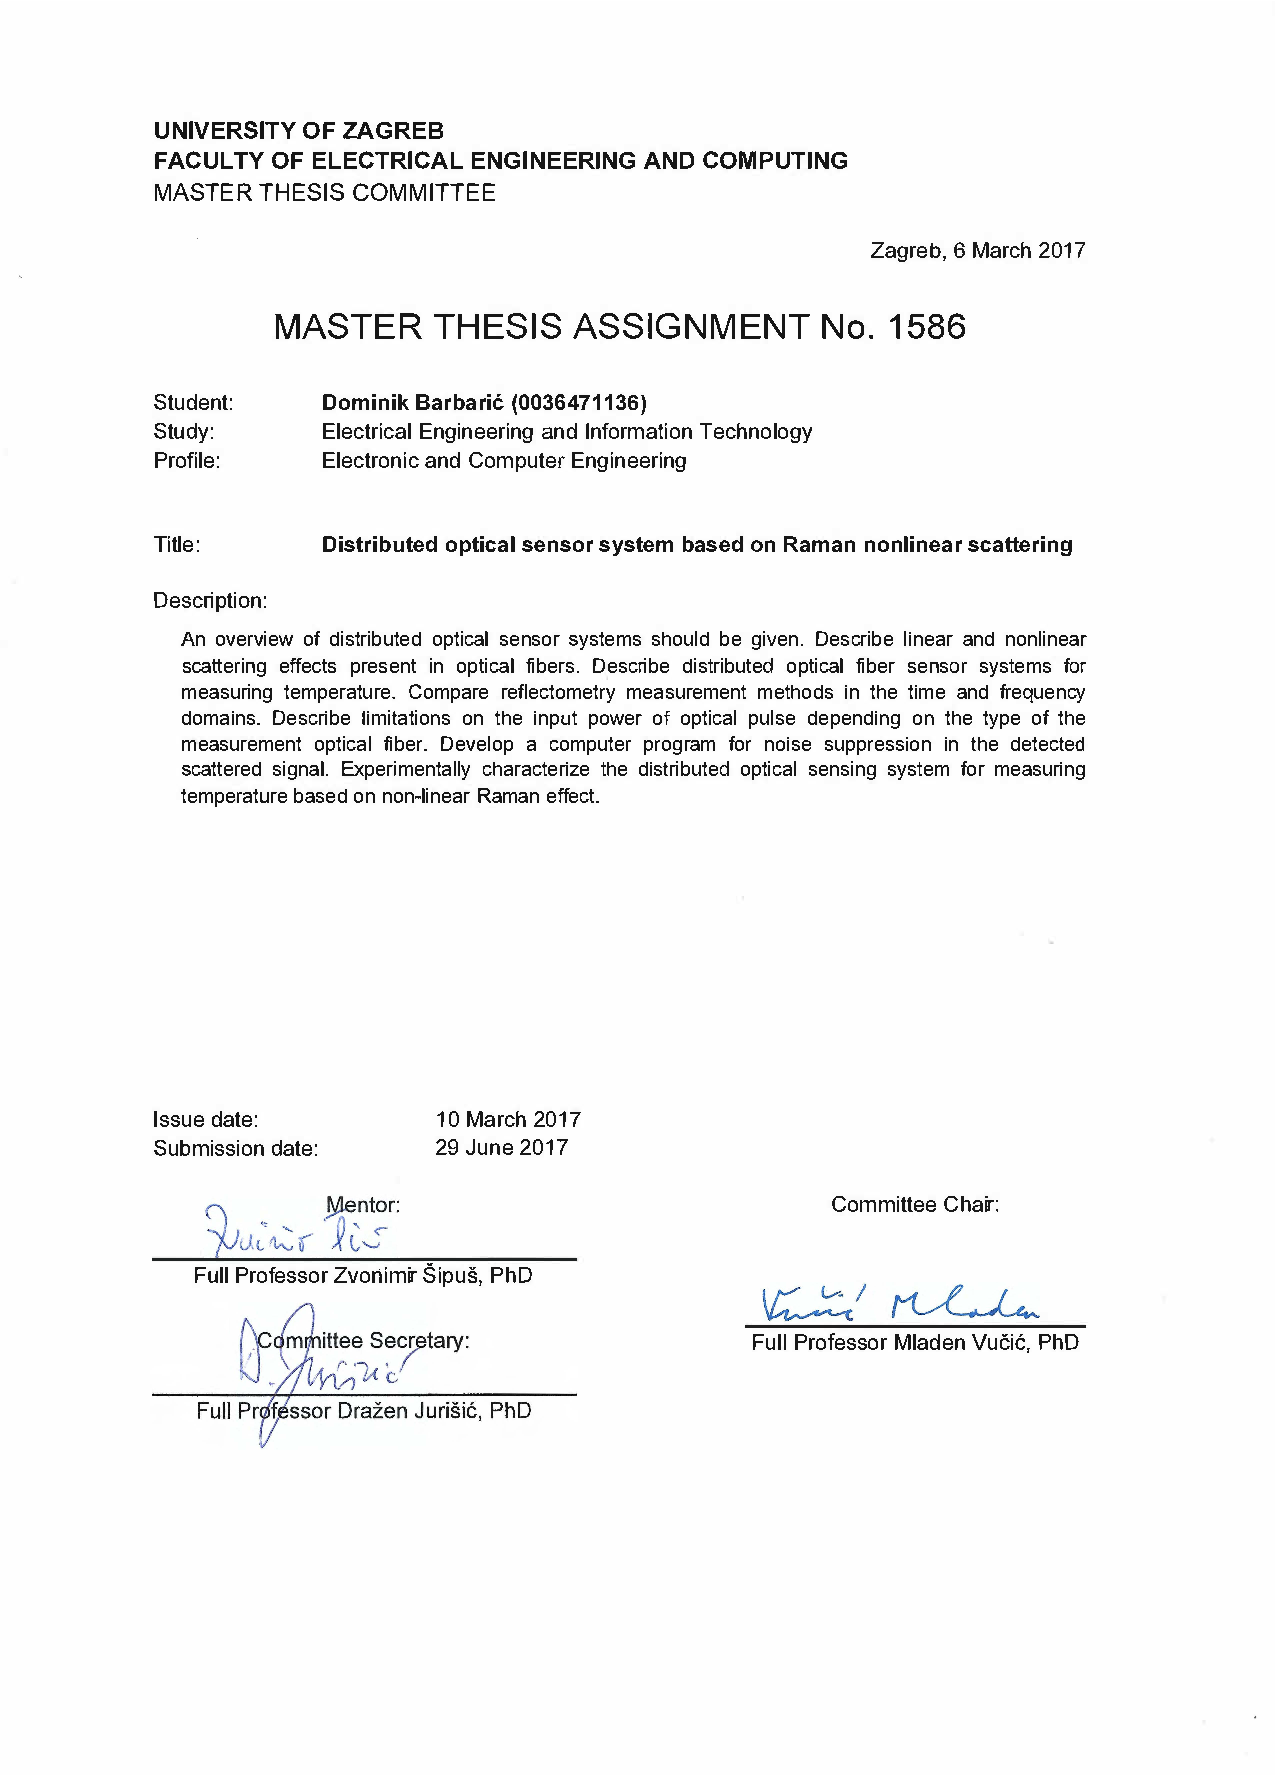
\includepdf[pages={1}]{diplomski_zadatak_eng.pdf}
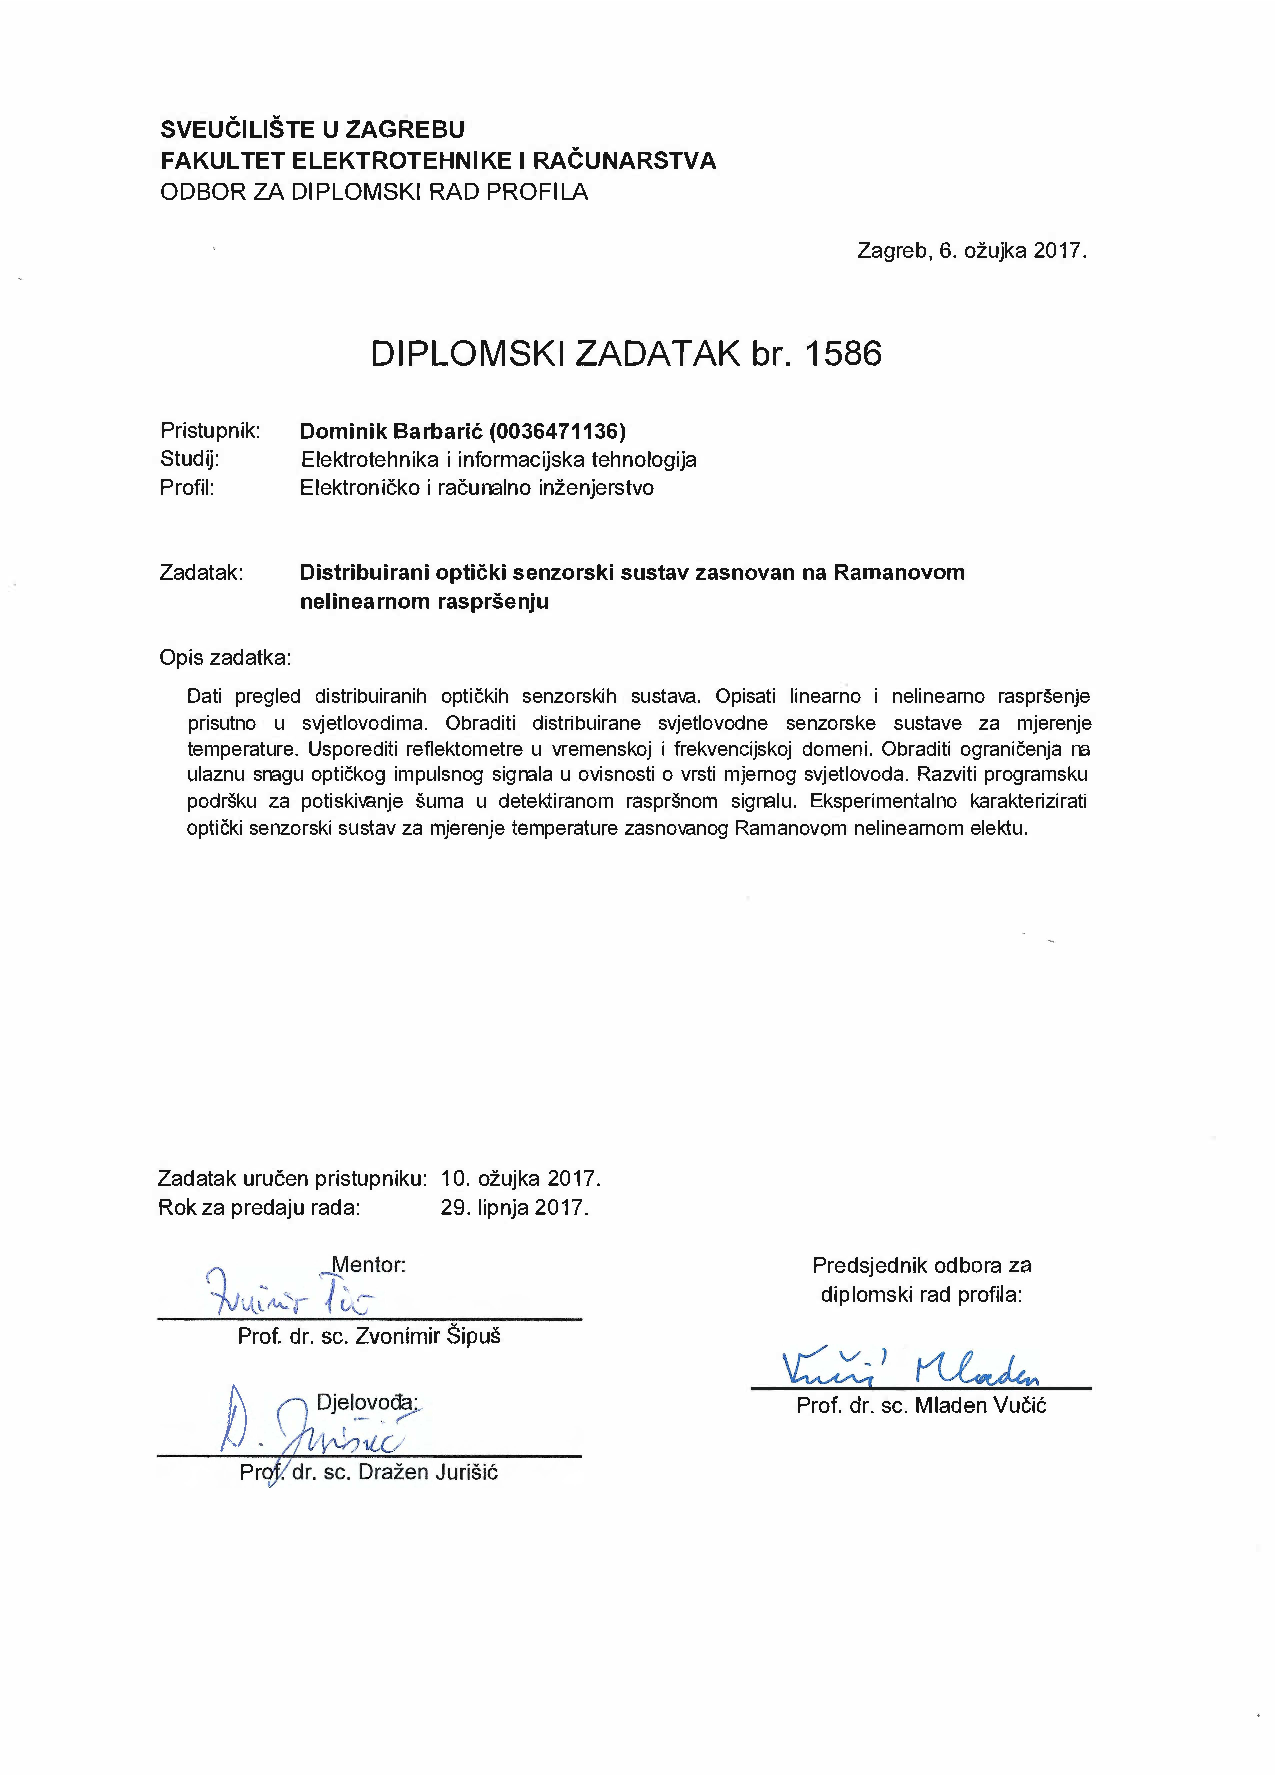
\includepdf[pages={1}]{diplomski_zadatak_hrv.pdf}

\zahvala{}

\tableofcontents

\subimport{./chapters/}{introduction.tex}
\subimport{./chapters/fibres/}{fibres.tex}
\subimport{./chapters/sensing_method/}{sensing_method.tex}
\subimport{./chapters/setup/}{setup.tex}
\subimport{./chapters/data_processing/}{data_processing.tex}
\subimport{./chapters/results/}{results.tex}
\subimport{./chapters/discussion/}{discussion.tex}
\subimport{./chapters/}{conclusion.tex}

\bibliography{literatura}

\begin{abstract}
A distributed temperature sensing systems is implemented and described. The system is based on optical time-domain reflectometry, and Raman scattering effect. The basic theory of optical fibres and their application in communication systems is described, along with significant linear and non-linear fibre-optical effects. Two reflectometric methods for characterizing optical fibres are explained. The implemented system is thoroughly described, calibrated and tested. Results obtained using two different laboratory setups, based on single-mode and multi-mode fibres, are presented. System performance is discussed, and methods for future enhancements are suggested.

\keywords{Distributed temperature sensor, Fibre-optical sensor, Optical time-domain reflectometry, Raman scattering, Brilloiun scattering}
\end{abstract}

\begin{sazetak}
Implementiran je i opisan distribuirani sustav za mjerenje temperature. Sustav se zasniva na metodi optičke reflektometrije u vremenskoj domeni i efektu Ramanovog raspršenja. Opisane su osnove teorije svjetlovoda i njihove primjene u komunikacijskim sustavima, kao i značajni linearni i nelinearni efekti u svjetlovodima. Objašnjene su dvije reflektometrijske metode za karakterizaciju svjetlovoda. Implementirani sustav je potanko opisan, kalibriran i ispitan. Predstavljeni su rezultati dobiveni dvama postavima, zasnovanima na jednomodnim i višemodnim svjetlovodima. Raspravljene su mogućnosti sustava, a predložene su i metode za daljnju nadogradnju.

\kljucnerijeci{Distribuirani svjetlovodni senzor, Svjetlovodni senzor, Optički reflektometar u vremenskoj domeni, Ramanovo raspršenje, Brillouinovo raspršenje}
\end{sazetak}

\end{document}
